\documentclass[a4paper]{scrreprt}

\usepackage[T1]{fontenc}
\usepackage[ngerman]{babel}     % deutsche Silbentrennung
\usepackage[utf8x]{inputenc}    % wegen deutschen Umlauten & UTF-8
\usepackage{lmodern}		% Schönere Schriftart
\usepackage{graphicx}           % Grafikpaket laden
\usepackage{amsmath,amssymb}    % Mathe
\usepackage{tikz}               % Zeichungen
\usepackage{hyperref}		% Links
\hypersetup{			% Link-Formatierung entfernen & pdf-Inforamtionen setzten
	pdfauthor={Maximilian Awiszus, Holger Ebhart, Lidia Grigoriev, Paul Jungeblut, Philipp Kern  und Matthias Schimek},
	pdftitle={Visualizing Trends - Was verrät uns Twitter?},
	colorlinks,
	citecolor=black,
	filecolor=black,
	linkcolor=black,
	urlcolor=black
}
\usepackage{microtype}		% font expansion

\title{Visualizing Trends\\Was verrät uns Twitter?}
\author{Maximilian Awiszus\and Holger Ebhart\and Lidia Grigoriev\and Paul Jungeblut\and Philipp Kern\and Matthias Schimek}

\begin{document}
	\maketitle
	\tableofcontents
	\chapter{Lastenheft}
		\input{include/lastenheft.tex}
	\chapter{Pflichtenheft}
		\documentclass[a4paper]{scrreprt}
	
\usepackage[T1]{fontenc}
\usepackage[ngerman]{babel}     % deutsche Silbentrennung
\usepackage[utf8x]{inputenc}    % wegen deutschen Umlauten & UTF-8
\usepackage{lmodern}		% Schönere Schriftart
\usepackage{graphicx}           % Grafikpaket laden
\usepackage{amsmath,amssymb}    % Mathe
\usepackage{tikz}               % Zeichungen
\usepackage{hyperref}		% Links
\hypersetup{			% Link-Formatierung entfernen & pdf-Inforamtionen setzten
	pdfauthor={Maximilian Awiszus, Holger Ebhart, Lidia Grigoriev, Paul Jungeblut, Philipp Kern  und Matthias Schimek},
	pdftitle={Visualizing Trends. Was verrät uns Twitter?},
	colorlinks,
	citecolor=black,
	filecolor=black,
	linkcolor=black,
	urlcolor=black
}
\usepackage{microtype}		% font expansion
\usepackage{enumerate}

\title{Praxis der Softwareentwicklung:\\Visualizing Trends. Was verrät uns Twitter?}
\subtitle{Pflichtenheft}
\author{Maximilian Awiszus\and Holger Ebhart\and Lidia Grigoriev\and Paul Jungeblut\and Philipp Kern\and Matthias Schimek}
\date{
\includegraphics[width=.3\textwidth]{img/logo.pdf}\\\vspace{3mm}WS 2014/15}

\begin{document}
	\maketitle
	\tableofcontents
	\chapter{Einleitung}
		% vollständige Beschreibung der Aufgabenstellung.

	\chapter{Zielbestimmungen}
		% Beschreibt die Funktionalität der zu entwickelnden Systemkomponente. 
% o Musskriterien: Mindestanforderungen, gehen aus Aufgabenstellung hervor. 
% o Wunschkriterien: Von den Gruppen selbst definierte, zusätzliche Funktionalität. 
% o Abgrenzungskriterien: Was gehört nicht zum Funktionsumfang? (vgl. auch Produkteinsatz) 

\section{Musskriterien}
\begin{itemize}
	\item Es soll ein Programm entwickelt werden, dass Twitterdaten (mittels Streaming- und Search-API) nach verifizierten Nutzern durchsucht und diese speichert.
	\item Zu Tweets von verifizierten Accounts sollen Retweets geografisch gruppiert und gezählt werden.
	\item Dazu soll einzelnen Accounts eine geografische Position und eine thematische Kategorie zugeordnet werden.
	\item Es sollen interaktiv Anfragen an das System gestellt werden können: Anfragen bestehen zum Beispiel aus einer Kategorie und einem Land. Damit soll die weltweite geografische Ausbreitung von Tweets mit diesen Eigenschaften grafisch dargestellt werden (siehe \cref{sec:Produktfunktionen}).
	\item Die Interaktion mit dem System soll über eine intuitiv bedienbare grafische Benutzeroberfläche geschehen. Diese soll neben den Auswahlhilfen eine Weltkarte sowie weitere Statistiken zeigen.
	\item Über die Benutzeroberfläche sollen Accounts manuell kategorisiert und lokalisiert werden können.
\end{itemize}

\section{Wunschkriterien}
Folgende Auflistung zeigt die Wunschkriterien in absteigender Priorität.
\begin{enumerate}
	\item Es soll möglich sein, nicht verifizierte Benutzer einzugeben, sodass die Ausbreitung ihrer Tweets analysiert werden kann.
	\item Visualisierung von Datenströmen auf der Karte.
	\item Eine Visualisierung der Analyseergebnisse mit Schwerpunkt auf der zeitlichen Entwicklung sowie weiterer Statistiken wie der Häufigkeit bestimmter Kategorien in verschiedenen Ländern.
	\item Eine hierarchische Einteilung der Regionen in Ergänzung zur Analyse pro Land. So könnte zum Beispiel pro Kontinent  visualisiert werden.
	\item Exportfunktion für Analyseergebnisse.
\end{enumerate}

\section{Abgrenzungskriterien}
\begin{itemize}
	\item Es werden Retweets pro Account, nicht pro Tweet analysiert. Daher wird es nicht möglich sein, einzelne Tweets zu analysieren.
	\item Es handelt sich um ein Analyseprogramm, nicht um ein Lokalisierungsprogramm. Zur Lokalisierung soll ein existierender Webservice genutzt werden.
	\item Die Analyse beruht nicht auf dem Inhalt der Tweets (Hashtags, etc.) sondern ausschließlich auf der dem Account zugeordneten Kategorie und Ort.
\end{itemize}

	\chapter{Produkteinsatz}
		% Beschreibt  Einsatzgebiete,  Zielgruppe  und  Betriebsbedingungen  sowie  notwendige Hard‐ und Software.
\section{Einsatzgebiet}
Die Software wird dazu verwendet die Anzahl der Retweets einer Kategorie von Tweets in einem Land in anderen Ländern zu analysieren. Einsatzgebiete sind somit u.a.:
\begin{itemize}
	\item Statistik
	\item Marktforschung
	\item Privat
\end{itemize}
\section{Zielgruppe}
Entsprechend oben genannter Einsatzgebiete richtet sich die Anwendung an folgende Zielgruppen:
\begin{itemize}
	\item Meinungsforscher
	\item Journalisten
	\item Privatpersonen
\end{itemize}
\section{Betriebsbedingungen}
Da die Anwendung aus Server und Client besteht muss für die Betriebsbedingungen unterschieden werden.
\subsection{Client}
\begin{itemize}
				\item Bei der aus Abschnitt \ref{sec:empfohleneHardware} gegebener Hardware darf die Anzahl parallel laufender GUIs 100 Instanzen nicht überschreiten.
\end{itemize}
\subsection{Server}

	\chapter{Produktumgebung}
		% Notwendige Hard‐ und Software.
\section{Software}
   \begin{itemize}
      \item Java Runtime Environement SE 1.7 oder höher
      \item MySQL-Datenbank
      \item Betriebssystem z.B. Windows, Linux, MacOS
   \end{itemize}
\section{Hardware}
\label{sec:empfohleneHardware}
   \subsection{Server}
	Minimalanforderungen:
   \begin{itemize}
      \item Hauptspeicher 4 GB
      \item freier Festplattenspeicher 20 GB
      \item Mindestens 2 GHz Multicore-Prozessor
   \end{itemize}
   Empfohlene Hardware:
   \begin{itemize}
      \item Hauptspeicher 8 GB
      \item freier Festplattenspeicher 100 GB
      \item Mindestens 2-3 GHz Quadcore-Prozessor
   \end{itemize}
   \subsection{Client}
   	Minimalanforderungen:
   \begin{itemize}
      \item Hauptspeicher 2 GB
      \item freier Festplattenspeicher 100 MB GB
      \item Mindestens 1 GHz Prozessor
   \end{itemize}
   Empfohlene Hardware:
   \begin{itemize}
      \item Hauptspeicher mind. 4 GB
      \item freier Festplattenspeicher 200 MB
      \item Mindestens 2 GHz Multicore-Prozessor
   \end{itemize}
\section{Schnittstellen}
   \begin{itemize}
   \item Webschnittstelle (Internetzugang) mindestens 4 MB/s, empfohlen 16 MB/s
   \end{itemize}
	\chapter{Produktfunktion}
		% Detailliertere  Beschreibung  der  Funktionalität,  wiederum  gegliedert  in Grundfunktionen und optionale Funktionen. 

Die Beschreibung der Funktionalität gliedert sich in Grundfunktionen und optionale Funktionen.

\section{Grundfunktionen}

Die Grundfunktionen der Anwendung gliedern sich in verschiedene Bereiche.

%\subsection{Allgemeine Funktionalität}
%\begin{enumerate}[align=left, label={\textbf{\textbackslash F00\arabic*0\textbackslash}} ]
%	\item Start des Programms \\
%	Bei Start des Programms wird die leere Weltkarte angezeigt.
%	\begin{itemize}
%		\item Hier könnte auch Ihre Werbung stehen ...
%	\end{itemize}


%\end{enumerate}
\subsection{Auswahl der gewünschten Daten} \label{sec:Produktfunktionen}
\begin{enumerate}[ align=left, label={\textbf{\textbackslash F10\arabic*0\textbackslash}} ]
	\item \textbf{Auswahl der Kategorien} \label{PF:KategorienAuswahl}\\ 
	Die verschiedenen Kategorien werden angezeigt. Man kann durch die Auswahl navigieren und eine oder mehrere Kategorien auswählen. Hierfür kann eine Suchfunktion genutzt werden ($\rightarrow$ \ref{PF:Suchfunktion}). 
	\item \textbf{Auswahl der Ortsbeschränkung} \label{PF:OrtAuswahl} \\
	Die verschiedenen Orte werden angezeigt. Man kann durch die Auswahl navigieren und einen oder mehrere Orte auswählen. Hierfür kann eine Suchfunktion genutzt werden ($\rightarrow$ \ref{PF:Suchfunktion}). 
	\item \textbf{Manuelles Hinzufügen weiterer Accounts} \label{PF:AccountHinzufügen} \\
	Mittels der Suchfunktion ($\rightarrow$ \ref{PF:Suchfunktion}) können weitere Accounts einzeln zur Auswahl hinzugefügt werden, sofern diese in der Datenbank hinterlegt sind.
	\item \textbf{Suchfunktion innerhalb des Auswahlprozesses} \label{PF:Suchfunktion} \\
	Es kann nach Kategorien, Orten und Benutzern gesucht werden, die bereits in der Datenbank vorhanden sind. Die Funktionalität unterscheidet sich je nach der Art des gesuchten Objekts. In allen Fällen wird eine Liste mit Vorschlägen abhängig vom gerade eingegebenen Suchbegriff angezeigt. 
	\item \textbf{Aktualisierung der Anfrage} \label{PF:Absenden} \\
	Bei Änderung der Anfrageparameter werden die Daten automatisch ausgewertet und nach einer gewissen Latenzzeit angezeigt.
\end{enumerate}	
\subsection{Visualisierung der Daten}	
Für die Visualisierung der Daten bestehen folgende Funktionen.
\begin{enumerate}[ align=left, label={\textbf{\textbackslash F20\arabic*0\textbackslash}} ]	
	\item \textbf{Anzeige der grafisch aufbereiteten Daten} \label{PF:Visualisieren}\\
	Die Daten der aktuellen Anfrage werden grafisch aufbereitet in der Karte dargestellt.
	\begin{itemize}
		\item Einfärben der Karte ($\rightarrow$ \ref{PF:EinfärbenKarte}).
		\item Detaillierte Informationen bezüglich einzelner Orte ($\rightarrow$ \ref{PF:DetailsKarte}).
	%	\item Wahl des Beobachtungszeitraums ($\rightarrow$ \ref{PF:WahlZeitraum}).
	%	\item Anzeige von Veränderungen des Tweet-Retweet-Verhaltens über einen Zeitraum ($\rightarrow$ \ref{PF:Diff})
	\end{itemize}
	
	\item \textbf{Einfärben der Karte} \label{PF:EinfärbenKarte} \\
	Die Länder/Regionen werden auf der Karte bezüglich der Tweet-Retweet-Intensität unterschiedlich eingefärbt. Hierbei handelt es sich um relative Daten, um Bevölkerungsunterschiede auszugleichen.
	\item \textbf{Detaillierte Informationen bezüglich einzelner Orte} \label{PF:DetailsKarte} \\
	Beim Bewegen des Mauszeigers über einen Ort werden detaillierte Informationen wie Anzahl der Retweets über die Tweet-Retweet-Beziehung der aktuellen Anfrage an diesem Ort angezeigt. Diese Option kann deaktiviert werden.
	
	
	\item \textbf{Anzeige mittels Datenblatt} \label{PF:AnzeigeDatenblatt} \\
	Die relevanten Daten der Anfrage werden in Tabellenform dargestellt. Zu einem Ort-Kategorie-Paar können die zugehörigen Accounts aufgelistet werden.
	

\end{enumerate}

\subsection{Navigation auf der Weltkarte}
\begin{enumerate}[ align=left, label={\textbf{\textbackslash F30\arabic*0\textbackslash}} ]
	\item \textbf{Navigation auf der Karte} \label{PF:Navigation} \\
	Es ist möglich die Karte zu verschieben.
	\item \textbf{Zoomen} \label{PF:Zoomen} \\
	Die Ansicht auf die Karte kann, innherhalb gewisser Grenzen, vergrößert und verkleinert werden.
\end{enumerate}	
\subsection{Manuelle Bearbeitung der Datenbank}
Durch den Benutzer können einige Änderungen der in der Datenbank  gespeicherten Daten vorgenommen werden. Diese Funktionen müssen gegebenenfalls eingeschränkt werden, sollte die Anwendung öffentlich verwendet werden.
\begin{enumerate}[ align=left, label={\textbf{\textbackslash F40\arabic*0\textbackslash}}]
	\item \textbf{Kategorie eines Accounts ändern}  \label{PF:KategorieAendern} \\
	Die Kategorie eines gespeicherten Accounts kann in eine schon in der Datenbank vorhandene Kategorie geändert werden.
	\item \textbf{Ort eines Accounts ändern} \label{PF:OrtAendern}\\
	Der Ort eines Account kann in einen schon in der Datenbank vorhandenen Ort geändert werden.
	\item \textbf{Account hinzufügen} \label{PF:AccountHinzu} \\
	Es kann ein Twitter-Account, sofern dieser existiert, zu der Liste der mitgelesenen Twitter-Accounts hinzugefügt werden, auch wenn dieser nicht verifiziert ist.
\end{enumerate}

\section{Optionale Funktionalität}
Die optionalen Funktionen sind nach absteigender Priorität aufgelistet.
\begin{enumerate}[ align=left, label={\textbf{\textbackslash F50\arabic*0\textbackslash}}]
	\item \textbf{Anzeigen von Veränderungen  zwischen zwei Zeitpunkten} \label{PF:Diff} \\
	Die Unterschiede in der Tweet-Retweet-Beziehung können zwischen zwei, innerhalb gewisser Grenzen, wählbaren Zeitpunkten grafisch dargestellt werden.
	\item \textbf{Wahl des Beobachtungszeitraums} \label{PF:WahlZeitraum} \\
	Der Zeitraum, für welchen die Tweet-Retweet-Beziehung dargestellt werden soll, kann innerhalb gewisser Grenzen und mit diskreten Zeitpunkten ausgewählt werden.
	\item \textbf{Allgemeine Suchfunktion} \label{PF:AllgSuche} \\
	Es wird eine allgemeine Suchfunktion angeboten. Hier kann nach beliebigen Begriffen gesucht werden. Die  Daten, welche zum jeweiligen Begriff in der Datenbank verfügbar sind, werden angezeigt.
	\item  \textbf{Sicherung von Ergebnissen} \label{PF:Sicherung} \\
	Die zu einer Anfrage erstellten Datenblätter und Kartenanzeigen können in geeignete Dateiformate exportiert und somit dauerhaft gespeichert werden.
	\item \textbf{Feingliederung der Auswahlmöglichkeiten} \\
	Es ist innerhalb einer größeren Anfrage möglich, einzelne Kategorien auf eine Teilmenge der insgesamt ausgewählten Orte zu beschränken. Man kann somit beispielsweise die Anfrage nach der Kategorie \emph{Musiker} auf den Ort \emph{Irland} einschränken und  derselben Anfrage noch die Kategorie \emph{Politiker} eingeschränkt auf den Ort \emph{Deutschland} hinzufügen.
	\item \textbf{Verknüpfung mit Twitteraccount} \label{PF:Verknuepfung} \\
	Ein Account in der Datenbank wird mit seinem Twitterprofil verknüpft. Wird der Account beispielsweise über die allgemeine Suchfunktion ($\rightarrow$ \ref{PF:AllgSuche}) gesucht und aufgerufen, werden Informationen aus der Timeline des Accounts angezeigt. 
	\item \textbf{Weitere Informationen zu Kategorien und Orten} \label{PF:WeiterInfos} \\
	Wird ein Ort oder eine Kategorie über die Suchfunktion ($\rightarrow$ \ref{PF:AllgSuche}) gesucht und aufgerufen, werden zusätzliche Informationen, die beispielsweise von wikipedia.org stammen, angezeigt.
	
	\item \textbf{Weitere Statistiken} \label{PF:Statistiken} \\
	Es werden noch weitere Statistikfunktionen und Anzeigeoptionen angeboten.
\end{enumerate}

	\chapter{Produktdaten}
		% Anfallende Daten außerhalb des Quellcodes.
\begin{itemize}
\section{GUI}
	\item[/PD1010/]Kartendaten der Länder
	\item[/PD1020/]Vom Benutzer hinzugefügte Accounts
	\item[/PD1030/]Namen aller Kategorien
	
\section{Server-Datenbank}
	\item[/PD2010/]zertifizierte Twitter-Accounts	
	\item[/PD2020/]Anzahl der Retweets pro Twitter-Account, getrennt nach Zeit und Ort
	\item[/PD2030/]Alle Twitter-Accounts zuweisbaren Kategorien
	\item[/PD2040/]Alle Orte
	\item[/PD2050/]Kategorie der zertifizierten Twitter-Accounts
	\item[/PD2060/]Lokalität der zerfifizierten Twitter-Accounts

\section{Server-Crawler}
	\item[/PD3010/]Zugangsdaten zu Twitter
\end{itemize}% Anfallende Daten außerhalb des Quellcodes.

	\chapter{Systemmodell}
		% Grobe  Architekturbeschreibung  durch  Bausteine/Komponenten  (Kein  detailliertes Klassendiagramm).

Das Projekt soll aus drei separaten Programmen bestehen. Es soll dabei keine Kommunikation untereinander stattfinden. Stattdessen greifen alle auf eine gemeinsame Datenbank zu. Eine Darstellung der drei Komponenten ist in Abbildung~\ref{c:systemmodell} zu finden.

\begin{figure}[h]
	\centering
	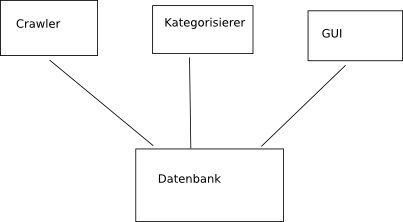
\includegraphics{img/systemmodell.png}
	\caption{Das Systemmodell}
	\label{c:systemmodell}
\end{figure}

\begin{description}
	\item[Crawler] Aufgabe des Crawlers ist es Mithilfe der Twitter-Stream- und Search-API die Twitterdaten zu sammeln. Es sollen verifizierte Benutzer und Retweets von Tweets dieser Nutzer gefunden werden. Diese Daten sollen noch im Crawler lokalisiert werden, bevor sie in der Datenbank abgespeichert werden.
	\item[Kategorisierer] Um den Crawler so leichtgewichtig wie möglich zu halten, werden die gefunden Accounts von einer weiteren Anwendung, dem Kategorisierer kategorisiert. Unabhängig vom Crawler sucht er in der Datenbank nach Accounts, denen noch keine Kategorie zugeordnet wurde. Anhand der Daten aus der DMOZ-Datenbank sollen diese Accounts dann hierarchisch kategorisiert werden. Dabei können einem Nutzer mehrere Kategorien zugeordnet werden. Der Kategorisierer arbeitet also auf den vom Crawler gefunden Daten und vervollständigt diese.
	\item[GUI] Die GUI greift lesend auf die Datenbank zu und visualisiert die Daten anhand vom Nutzer gegebener Eingaben. Sie baut somit auf Crawler und Kategorisierer auf, welche jedoch unabhängig von der GUI sind. Es ist möglich über die GUI weitere Twitteraccounts (auch nicht verifizierte) in die Datenbank aufzunehmen. Dies ist die einzige Art der Kommunikation von der GUI zur Datenbank und darüber auch zum Crawler und Kategorisierer.
\end{description}



	\chapter{Produktleistungen}
		% Wenn vorhanden, Anforderungen an Laufzeitverhalten oder Speicherplatz.
\section{Speicher}
\subsection{Server}
Durch das Sammeln von Daten mit Crawlern fällt in den ersten Wochen eine beträchtliche Menge an Daten an. Mit der Zeit, wenn ein Großteil der verifizierten Accounts gelistet ist, steigt das Volumen der Datenbank nicht mehr so stark an. Es ist dann von einer \textbf{linearen Steigerung} des Datenaufkommens auszugehen. 
Dadurch, dass der Twitterstream in Realzeit mitgelesen wird kann es zu  kurzzeitigen Peeks kommen, in denen der benötigte Hauptspeicherplatz steigt (z.B. bei hoher Anzahl an Tweets von verifizierten Accounts). Im Normalbetrieb kann allerdings von einer \textbf{stets gleich hohen Auslastung} des Hauptspeichers ausgegangen werden.
\subsection{Client}
Für die Benutzerschnittstelle (GUI) wird \textbf{kaum Festplattenspeicher} benötigt, da nur Einstellungen und benutzerdefinierte Daten lokal gespeichert werden. Die restlichen Daten werden in einer zentralen Datenbank bereitgehalten und bei Bedarf abgerufen.
Um eine flüssige Kartendarstellung zu gewährleisten wird genügend Hauptspeicherplatz benötigt (siehe \ref{subsec:hardwareClient}).
\section{Laufzeit}
\subsection{Server}
Da durch den Crawler Daten von Twitter in Realzeit gesammelt werden, können sich Beschränkungen aufgrund von Rate- und Connecting-Limits der Twitter Schnittstellen ergeben. Das Erreichen dieser Limits soll so gut wie möglich verhindert werden, allerdings können sich Verzögerungen ergeben. Es kann auch vorkommen, dass es dem Crawler für eine bestimmte Zeit nicht mehr möglich ist, sich mit Twitter zu verbinden. Um dennoch möglichst viele Daten ab zu schöpfen, sollte der Crawler 24 Stunden, 7 Tage die Woche laufen.
\subsection{Client}
Bei der Anfrage von Daten können sich Beschränkungen von Webdiensten ergeben. Diese sollen so gering wie möglich gehalten werden, weshalb eine durchschnittliche \textbf{Anfragezeit von kleiner 1 Sekunde} angestrebt wird, falls die Daten schon in der eigenen Datenbank bereitliegen und von kleiner 3 Sekunden falls die Daten erst von einem Webdienst abgeholt werden müssen.
Aufgrund der Visualisierung der Datenströme über eine Karte streben wir eine \textbf{Ladezeit} des Programms von \textbf{kleiner 8 Sekunden} an.\\\\
Alle Daten beziehen sich auf die in Abschnitt \ref{sec:empfohleneHardware} empfohlene Hardware.
	\chapter{Bedienoberfläche}
		% Beschreibung der anvisierten Bedienoberfläche (z.B. durch einen Prototyp oder frei gezeichnet) und Erläuterung der Menüstruktur.

\section{Hauptfenster}

\begin{figure}[h]
	\centering
	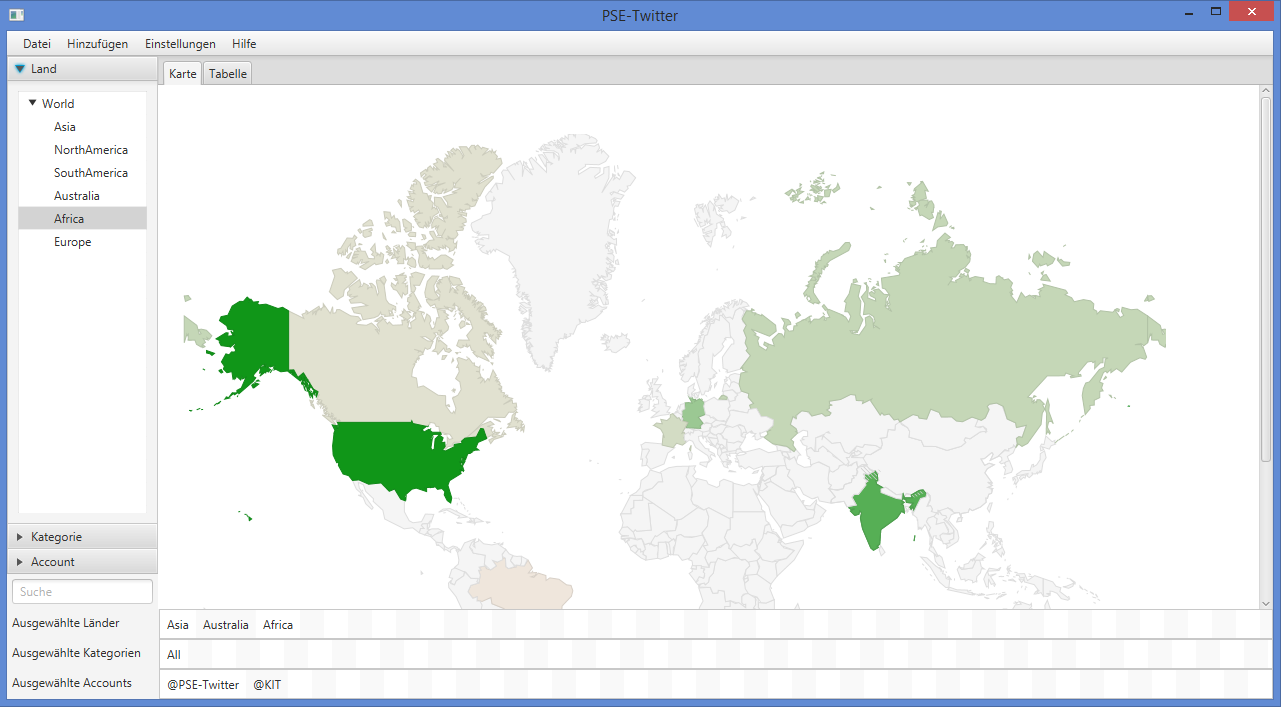
\includegraphics[width=0.9\textwidth]{img/DemoGUIMain.png}
	\caption{Hauptfenster}
	\label{c:Hauptfenster}
\end{figure}

\begin{description}
	\item[Landauswahl] In einer Baumstruktur werden Länder angezeigt. Die Auswahl einzelner Länder erfolgt durch Doppelklick auf das jeweilige Item.
	\item[Kategorienauswahl] Die Kategorien der DMOZ.org Datenbank werden als Baumstruktur angezeigt. Auswahl der Kategorien erfolgt durch Doppelklick auf das jeweilige Item.
	\item[Accountauswahl] In einer Liste werden Accounts (aus der eigenen Datenbank) angezeigt, die man ebenfalls per Doppelklick auswählen kann.
	\item[Suchfeld] In diesem Textfeld kann ein Begriff eingegeben werden. Je nach geöffnetem Fenster wird nach Land, Kategorie oder Account gesucht.
	\item[Länderübersicht] Eine Liste der bereits ausgewählten Länder.
	\item[Kategorienübersicht] Eine Liste der bereits ausgewählten Kategorien.
	\item[Accountübersicht] Eine Liste der bereits ausgewählten Accounts.
	\item[Karte] Die Weltkarte zeigt zu Beginn nur die Umrisse der Länder. Nach Auswahl von Ländern, Kategorien oder Accounts wird die Karte je nach Verteilung der Retweets zur Auswahl eingefärbt.	
\end{description}

\section{Tabellenansicht}

\begin{figure}[h]
	\centering
	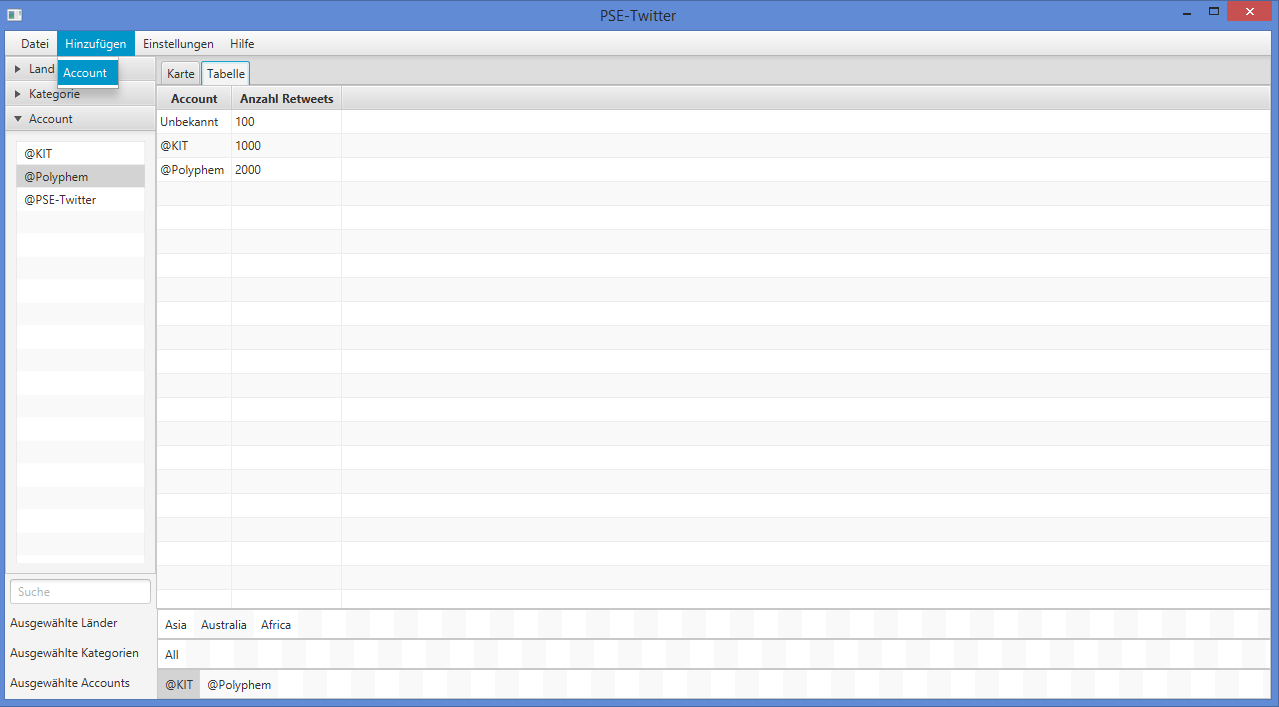
\includegraphics[width=0.9\textwidth]{img/DemoGUITabelleAddAccount.png}
	\caption{Tabellenansicht mit Menu}
	\label{c:Tabellenansicht mit Menu}
\end{figure}

\begin{description}
	\item[Hinzufügen-Menu] Menu-Eintrag, um einen weiteren (beliebigen) Twitter-Account hinzuzufügen. Klicken auf diesen Eintrag öffnet ein Fenster zum Hinzufügen eines Accounts.
	\item[Tabelle] Die Tabelle zeigt Informationen zu den einzelnen ausgewählten, zu Kategorien oder zu Ländern gehörenden Accounts.
\end{description}

\section{Fenster zum Hinzufügen von Accounts}

\begin{figure}[h]
	\centering
	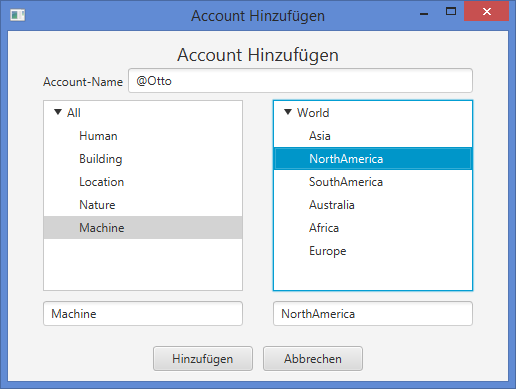
\includegraphics[width=0.9\textwidth]{img/DemoGUIAddAccount.png}
	\caption{Fenster zum Hinzufügen von Accounts}
	\label{c:Fenster zum Hinzufügen von Accounts}
\end{figure}

\begin{description}
	\item[Namensfeld] Textfeld zur Eingabe des Namens des hinzuzufügenden Accounts.
	\item[Hinzufügen-Button] Durch Drücken wird der eingegebene Account überprüft und gespeichert, sowie das Fenster geschlossen.
	\item[Abbrechen-Button] Dadurch wird der Hinzufügen-Vorgang unterbrochen und das Fenster geschlossen.
\end{description}

	\chapter{Qualitätszielbestimmungen}
		% Anforderungen  an  Stabilität,  Robustheit,  Leistungsfähigkeit  etc.  des Systems.  Dies  beinhaltet  auch  den  Umgang  mit  fehlerhaften  Eingabedaten  oder  fehlerhaften Konfigurationen.

	\chapter{Testfälle und Testszenarien}
		% Testfälle  für  die  einzelnen  Produktfunktionen,  die  alle  abgedeckt  sein müssen. Testszenarien für typische Anwendungsszenarien.

	\chapter{Entwicklungsumgebung}
		% Zur Entwicklung verwendete Hard‐ und Software. In der Pflichtenheft‐Phase soll  sich  das  Team  in  die  Werkzeuge  einarbeiten  und  sich  hier  vorläufig  festlegen.  Zu  diesen Werkzeugen zählen unter anderem ein UML‐Modellierungswerkzeug, IDE, Code‐Verwaltungssystem.

\section{Allgemein}
\begin{itemize}
	\item LaTeX
	\item Versionskontrolle (Git)
\end{itemize}
\section{Entwurf}
\begin{itemize}
	\item
\end{itemize}
\section{Implementierung}
\begin{itemize}
	\item Eclipse
	\item MySQL Workbench
\end{itemize}
\section{Validierung}
\begin{itemize}
	\item JUnit
	\item EclEmma
\end{itemize}
\section{Interne Kommunikation}
\begin{itemize}
	\item Email
\end{itemize}

	\chapter{Glossar}
		% Esentielle Begriffe.

\begin{description}

\end{description}

\end{document}

	\chapter{Entwurf}
		\documentclass[a4paper]{scrreprt}
	
\usepackage[T1]{fontenc}
\usepackage[ngerman]{babel}     % deutsche Silbentrennung
\usepackage[utf8x]{inputenc}    % wegen deutschen Umlauten & UTF-8
\usepackage{lmodern}		% Schönere Schriftart
\usepackage{graphicx}           % Grafikpaket laden
\usepackage{amsmath,amssymb}    % Mathe
\usepackage{tikz}               % Zeichungen
\usepackage{hyperref}		% Links
\hypersetup{			% Link-Formatierung entfernen & pdf-Inforamtionen setzten
	pdfauthor={Maximilian Awiszus, Holger Ebhart, Lidia Grigoriev, Paul Jungeblut, Philipp Kern  und Matthias Schimek},
	pdftitle={Visualizing Trends. Was verrät uns Twitter?},
	colorlinks,
	citecolor=black,
	filecolor=black,
	linkcolor=black,
	urlcolor=black
}
\usepackage{microtype}		% font expansion
\usepackage{enumerate}

\title{Praxis der Softwareentwicklung:\\Visualizing Trends. Was verrät uns Twitter?}
\subtitle{Pflichtenheft}
\author{Maximilian Awiszus\and Holger Ebhart\and Lidia Grigoriev\and Paul Jungeblut\and Philipp Kern\and Matthias Schimek}
\date{
\includegraphics[width=.3\textwidth]{img/logo.pdf}\\\vspace{3mm}WS 2014/15}

\begin{document}
	\maketitle
	\setcounter{tocdepth}{1}
	\tableofcontents

	\chapter{Einführung}
		% vollständige Beschreibung der Aufgabenstellung.
	
	\chapter{Datenbank}
	\label{chap:datenbank}
		\section{Datenbankzugriff}\label{sec:datenbankzugriff}
Die zentrale Komponente unseres Systems ist die Datenbank. In sie fügt der Crawler neue Datensätze ein und aktualisiert Vorhandene. Der Kategorisierer ist dafür zuständig die gefundenen Accounts nach der DMOZ.org Datenbank in Kategorien zu unterteilen. Die GUI wiederum ist die Komponente die die Daten aus der Datenbank ausliest und visualisiert. Gegebenenfalls kann sie auch Einträge hinzufügen, verändern beziehungsweise vervollständigen.
\\Da alle unsere drei Systemkomponenten lesend, sowie schreibend auf die Datenbank zugreifen, haben wir uns entschlossen ein Paket für den Datenbankzugriff für alle Komponenten zur Verfügung stellen. Dieses sogenannte mysql-Package ist dann für den Auf- und Abbau der Verbindung zur Datenbank zuständig, sowie für das Schreiben und Lesen in beziehungsweise aus der Datenbank. Es stellt für jede der drei Komponenten ein eigenes Interface zur Verfügung, sodass jede Komponente nur die für sie erlaubten Änderungen an der Datenbank vornehmen kann.
In \cref{fig:mysql-package} ist der Aufbau des mysql-Packages zu sehen. Das darin eingeschlossene result-Package stellt Objekt und Methoden zu Verfügung um die Ergebnisse aus der Datenbank zu speichern und zu verarbeiten.

\begin{figure}[h!]
	\centering
	\includegraphics[width=\textwidth,height=\textheight,keepaspectratio=true]{dia/uml_mysql-package}
	\caption{UML-Klassendiagramm des mysql-Packages}
	\label{fig:mysql-package}
\end{figure}

\begin{description}
	\item[AccessData] Klasse zur Verwaltung von Zugriffsdaten für die Datenbank.
	\item[DBConnection] Abstrakte Klasse die eine Verbindung zu einer Datenbank aufbaut und diese Verbindung auch wieder trennt.
	\item[DBIcrawler] Interface, welches die Methoden spezifizieren die der Crawler für den Datenbankzugriff benötigt.
	\item[DBIcategorizer] Interface, welches die Methoden spezifizieren die der Kategorisierer für den Datenbankzugriff benötigt.
	\item[DBIgui] Interface, welches die Methoden spezifizieren die die GUI für den Datenbankzugriff benötigt.
	\item[DBcrawler] Diese Klasse implementiert die Methoden des DBIcrawler Interfaces und stellt dem Crawler eine Datenbankverbindung zur Verfügung.
	\item[DBcategorizer] Diese Klasse implementiert die Methoden des DBIcategorizer Interfaces und stellt dem Kategorisierer eine Datenbankverbindung zur Verfügung.
	\item[DBgui] Diese Klasse implementiert die Methoden des DBIgui Interfaces und stellt dem der GUI eine Datenbankverbindung zur Verfügung.
	\item[Index] Als abstrakte Klasse stellt Index eine Möglichkeit zum Speichern des Datenbankindexes von Datenbankeinträgen zur Verfügung.
	\item[Account] In dieser Klasse werden einzelne Accounts verwaltet und gespeichert.
	\item[Retweets] In dieser Klasse werden nach Orten (und eventuell nach Daten) gruppierte Retweets verwaltet und gespeichert.
	\item[Tweets] In dieser Klasse werden nach Daten gruppierte Tweets verwaltet und gespeichert.
	\item[Location] In dieser Klasse werden einzelne Orte verwaltet und gespeichert.
	\item[Category] In dieser Klasse werden einzelne Kategorien verwaltet und gespeichert.
	\item[TweetsAndRetweets] Diese Klasse wird benutzt um zusammengefasste Daten der Datenbank an die GUI weiter zu leiten.
\end{description}

\section{ER-Modell}
Die Datenbank besteht aus sieben Tabellen, die über Fremdschlüssel miteinander in Relation stehen (s. \cref{fig:mysql-er}).
\begin{description}
	\item[accounts] Enthält alle verifizierten Accounts, die der Crawler im Twitter Stream mitgelesen hat, bzw. auch nicht verifizierte Accounts, die in der GUI hinzugefügt wurden. Dabei entspricht \emph{TwitterAccountId} der ID des Accounts in Twitter und \emph{id} ist ein Datenbank interner Primärschlüssel. Die Attribute \emph{Verified}, \emph{URL} und \emph{AccountName} entsprechen jeweils in Twitter hinterlegten Daten. \emph{Categorized} gibt an ob dieser Account bereits kategorisiert wurde und \emph{LocationId} Enthält den vom Loakaliserer berechneten zugehörigen Ort.
	\item[category] speichert die hierarchisch strukturierten (\emph{ParentId}) Kategorien.
	\item[accountCategory] Stellt die Relation zwischen	\emph{accounts} und \emph{category} in einer separaten Tabelle her, da einem Account mehrere Kategorien zugeordnet werden können.
	\item[location] Enthält die vom Lokalisierer ermittelten Orte, die jeweils \emph{Code} und \emph{Name} enthalten und auch per \emph{ParentId} hierarchisch gegliedert sein können.	
	\item[day] Enthält unterschiedliche Daten (\emph{Day}), die mittels \emph{Id} referenziert werden.
	\item[tweets] Beinhaltet die Anzahl der Tweets (\emph{Counter}) eines Accounts (\emph{AccountId}) an einem bestimmten Tag (\emph{DayId}).
	\item[retweets] Speichert die Anzahl der Retweets (\emph{Counter}) auf Tweets eines Accounts (\emph{AccountId}) an einem bestimmten Tag (\emph{DayID}) innerhalb eines bestimmten Lands bzw. Orts (\emph{LocationId}).
\end{description}
\begin{figure}[h!]
	\centering
	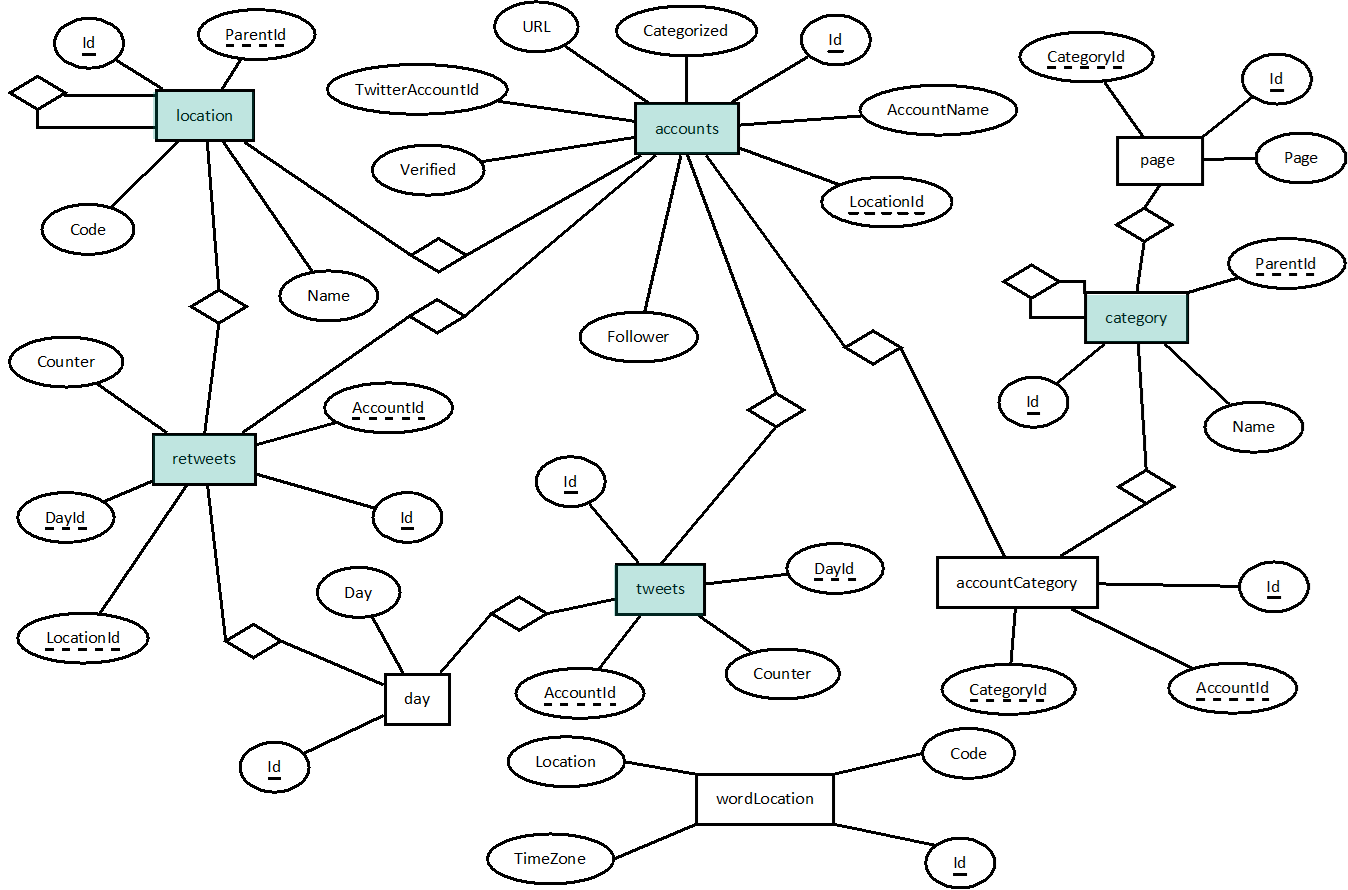
\includegraphics[width=\textwidth,height=\textheight, keepaspectratio=true]{dia/er}
	\caption{ER-Modell der MySQL-Datenbank}
	\label{fig:mysql-er}
\end{figure}

\section{Datenbankzugriff der GUI}
Da die GUI zur Visualisierung der Daten aus der Datenbank dient, ist es nötig, dass sie diese Daten in möglichst kompakter und vollständiger Form abrufen kann. Dazu stehen der GUI mehrere Möglichkeiten zur Verfügung die im Folgenden aufgelistet sind. Dabei sollen zum einen die Fähigkeiten der Datenbank ausgenutzt werden um Daten zusammenzufassen, zum Anderen sollen aber auch alle relevanten Daten einzeln zur Verfügung stehen.
\begin{description}
\item[Kategorien und Orte] Diese Informationen können jeweils als komplette Tabelle von der Datenbank geholt werden.
\item[Accounts] Mithilfe eines Account-Namens ist es möglich die AccountId herauszufinden. Außerdem kann mittels eines Worts nach Accounts gesucht werden, welche dieses Wort im Namen beinhalten.
\item[Tweets und Retweets] Um zu vorgegebenen Kategorien und Orten die Daten zu bekommen, sollen 4 Methoden zur Verfügung stehen. Im Folgenden werden jeweils nur die Tweets und Retweets von Accounts betrachtet, auf welche die Kategorie-Ort-Kombination/en passen.

\begin{itemize}
	\item Methoden welche über alle Kalenderdaten summieren:
	\begin{itemize}
		\item Eine Methode liefert jeweils die Summe der Tweets und Retweets pro Ort zurück, also für jeden Ort aus der Datenbank eine Summe von Tweets und eine Summe von Retweets.
		\item Eine weitere Methode liefert alle Accounts mit der Summe ihrer Tweets zurück auf die die Kategorie-Orts-Kombination passt. Dabei wird zu jeder Account-Orts Kombination eine Summe der Retweets mitgeliefert.
	\end{itemize}
	\item Methoden welche die Daten nach Kalenderdaten separieren:
	\begin{itemize}
		\item Eine Methode liefert für jede Ort-Datums Kombination, die Summe über alle Tweets und Retweets zurück, sodass dann zu jedem Ort zu jedem Datum eine Summe von Tweets und Retweets bekannt ist.
		\item Eine weitere Methode liefert alle betroffenen Accounts zurück und pro Account noch die Anzahl der Retweets pro Ort pro Tag und die Tweets pro Tag.
	\end{itemize}
\end{itemize}
Die Berechnungen werden so weit möglich in die Datenbank ausgelagert, sodass diese die Summation übernimmt. Dadurch kann die Geschwindigkeit der Datenbank ausgenutzt werden und die Ressourcen auf Client-Seite werden geschont.


\end{description}
	\chapter{Crawler}
	\label{chap:crawler}
		\section{Aufbau}

\subsection{Paketdiagramm}
In \cref{fig:crawler_package} ist die Grobstruktur des Crawlers als Paketdiagramm zu sehen.
\begin{figure}[h!]
	\centering
	\includegraphics[width=\textwidth,height=\textheight,keepaspectratio=true]{dia/crawler_package}
	\caption{Paketdiagramm des Crawlers}
	\label{fig:crawler_package}
\end{figure}

\begin{description}
\item[main] Dieses Paket beinhaltet die wesentliche Programmlogik.
\item[mysql] In diesem Paket sind Klassen, welche Methoden bereitstellen um auf eine MySQL-Datenbank zuzugreifen. Außerdem ist noch ein Paket mit Klassen zur Verwaltung von Twitter-Daten integriert.
\item[locate] Das locate-Paket dient zur Lokalisierung von Twitter-Accounts und Retweets mittels Webdiensten.
\item[java 1.8] Standard java 1.8 Bibliothek.
\item[twitter4j] twitter4j Bibliothek.
\end{description}

\subsection{Klassendiagramm}
Zum Sammeln von Daten von Twitter verwenden wir einen Crawler, welcher über die Twitter-API Daten sammelt. Dazu ist es nötig diese Daten zu empfangen, dann zu puffern und schlussendlich in die Datenbank zu schreiben. Allerdings müssen die Daten noch gefiltert werden, da wir nur Daten von verifizierten Twitter-Accounts (und manuell hinzugefügten) speichern. Sind die Daten gefiltert, werden sie vom Crawler noch lokalisiert. Das heißt, dass jedem Account beziehungsweise jedem Retweet eine Geoposition/Land zugeordnet wird. Ist dies erfolgt so werden die Daten in die Datenbank geschrieben.
\\ In \cref{fig:uml_crawler} ist der Aufbau des Crawlers anhand eines UML-Klassendiagramms spezifiziert.

\begin{figure}[h!]
	\centering
	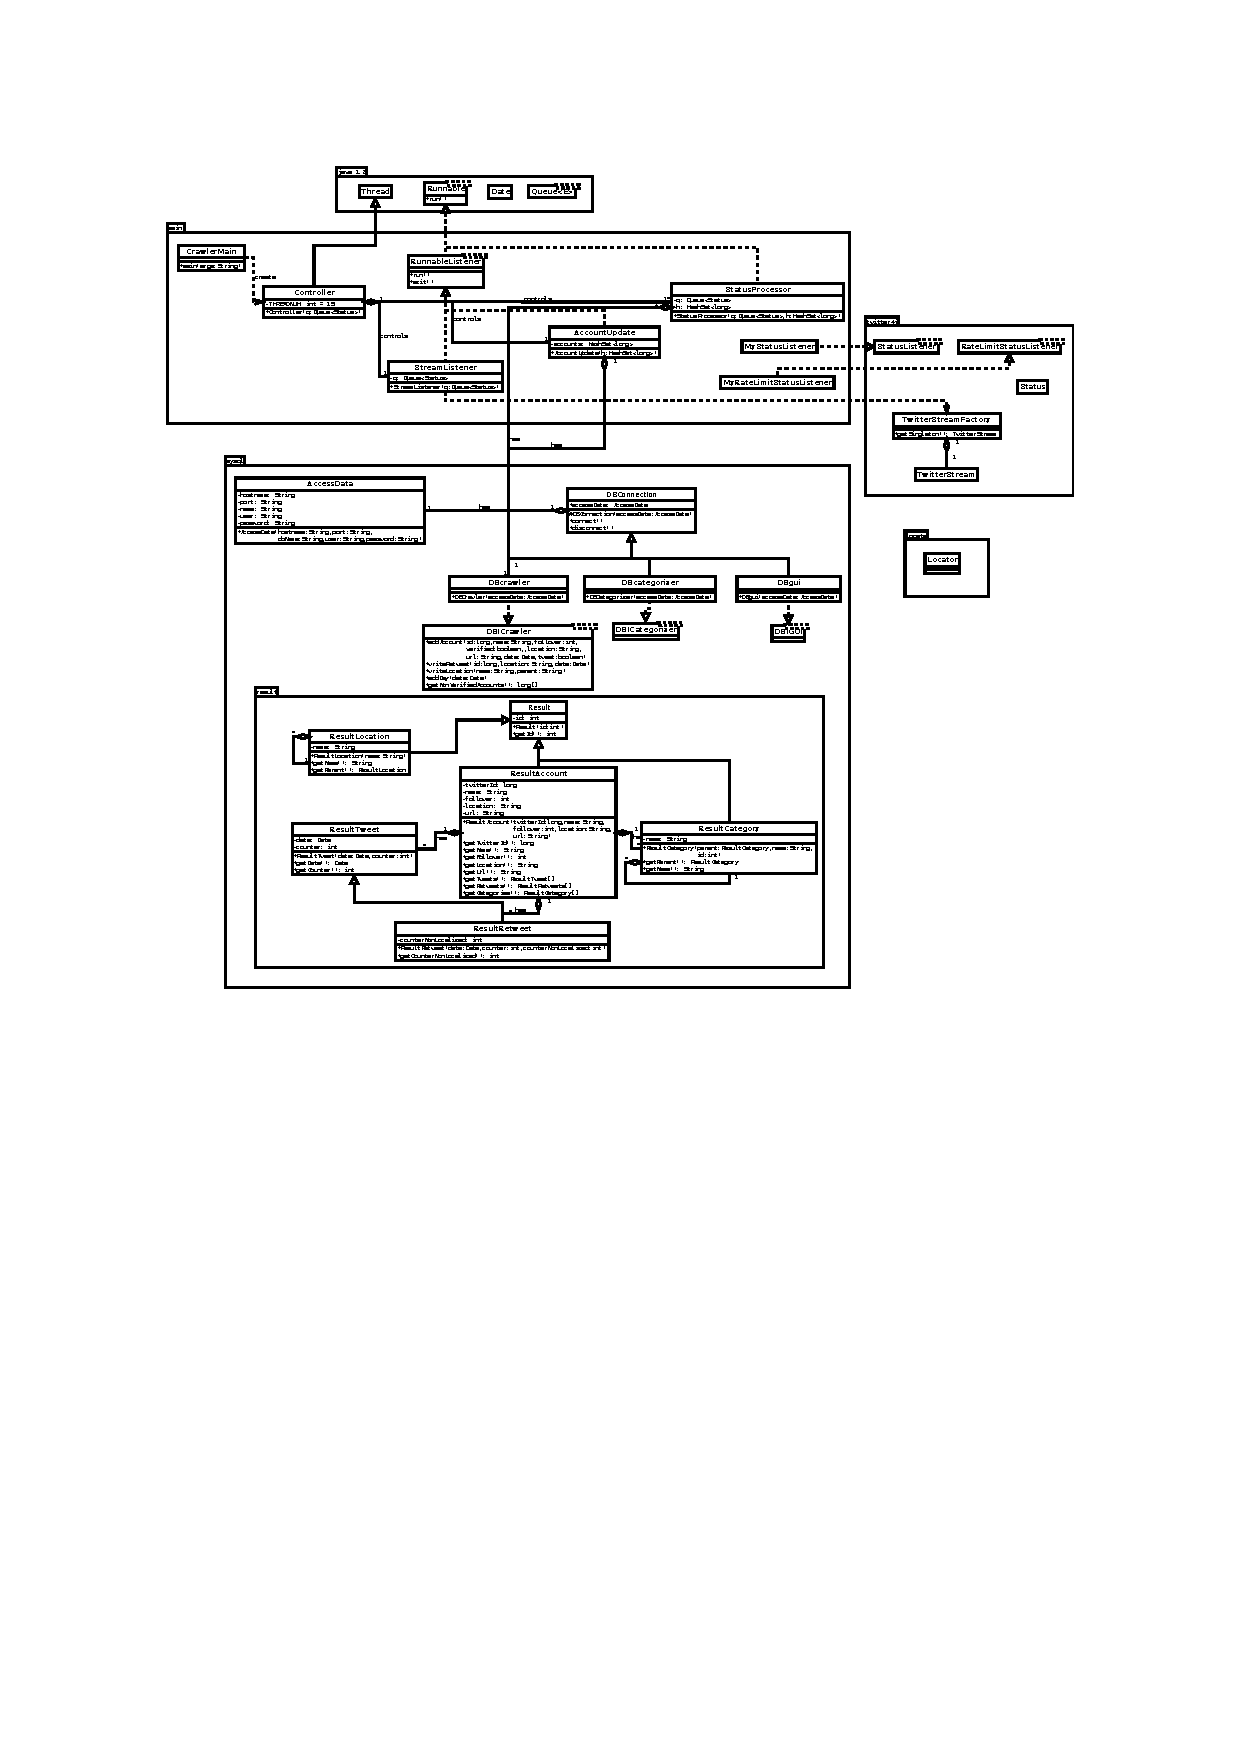
\includegraphics[width=\textheight,height=\textwidth,keepaspectratio=true,angle=-90]{dia/uml_crawler}
	\caption{UML-Klassendiagramm des Crawlers}
	\label{fig:uml_crawler}
\end{figure}

\begin{description}
\item[CrawlerMain] Klasse enthält die main-Methode zum Aufrufen des Programms. Sie überprüft die Eingabe für die Datenbankverbindung und startet einen Controller. Danach seht sie dem Benutzer über die Konsole zur Verfügung um das Programm zu überwachen.
\item[RunnableListener] Interface welches Runnable erweitert und zusätzlich noch eine exit-Methode fordert um Threads zu beenden.
\item[Controller] Diese Klasse koordiniert alle Aktionen die nötig sind um Daten bei Twitter abzuholen und in die Datenbank zu schreiben. Dazu startet sie einen StreamListener, ein AccountUpdate und mehrere StatusProcessors jeweils als Thread. Außerdem kontrolliert sie den Puffer und sorgt für ein sauberes Beenden des Programms indem alle Verbindungen ordnungsgemäß geschlossen und die Threads beendet werden.
\item[StreamListener] Stellt eine Verbindung zur Twitter-Streaming-API her und initialisiert einen MyStatusListener.
\item[AccountUpdate] Diese Klasse stellt eine Methode zur Verfügung um in der Datenbank periodisch nach Accounts zu suchen, welche manuell hinzugefügt wurden, nicht verifiziert sind, aber auch getracked werden sollen.
\item[StatusProcessor] Diese Klasse stellt die Funktionalität zur Filterung der Daten von Twitter zur Verfügung, welche sie aus dem Puffer nimmt. Außerdem bietet sie die Möglichkeit diese Daten in die Datenbank zu schreiben.
\item[MyStatusListener] Diese Klasse nimmt die Daten von Twitter entgegen und schreibt diese in einen Puffer.
\item[MyRateLimitStatusListener] Diese Klasse nimmt Meldungen von Twitter bezüglich RateLimits entgegen.
\item[Locator] Der Locator lokalisiert Accounts und Retweets mithilfe eines Webdienstes.
\end{description}

\section{Start des Crawlers}
Beim Starten des Crawlers werden sämtliche notwendigen Komponenten der Reihe nach gestartet. Dadurch wird garantiert, dass jede Komponente eine Umgebung vorfindet in der sie laufen kann und alle Ressourcen bereits zur Verfügung stehen. In \cref{fig:crawler_start} ist der Start des Crawlers beispielhaft mit 2 StatusProcessors dargestellt.

\begin{figure}[h!]
	\centering
	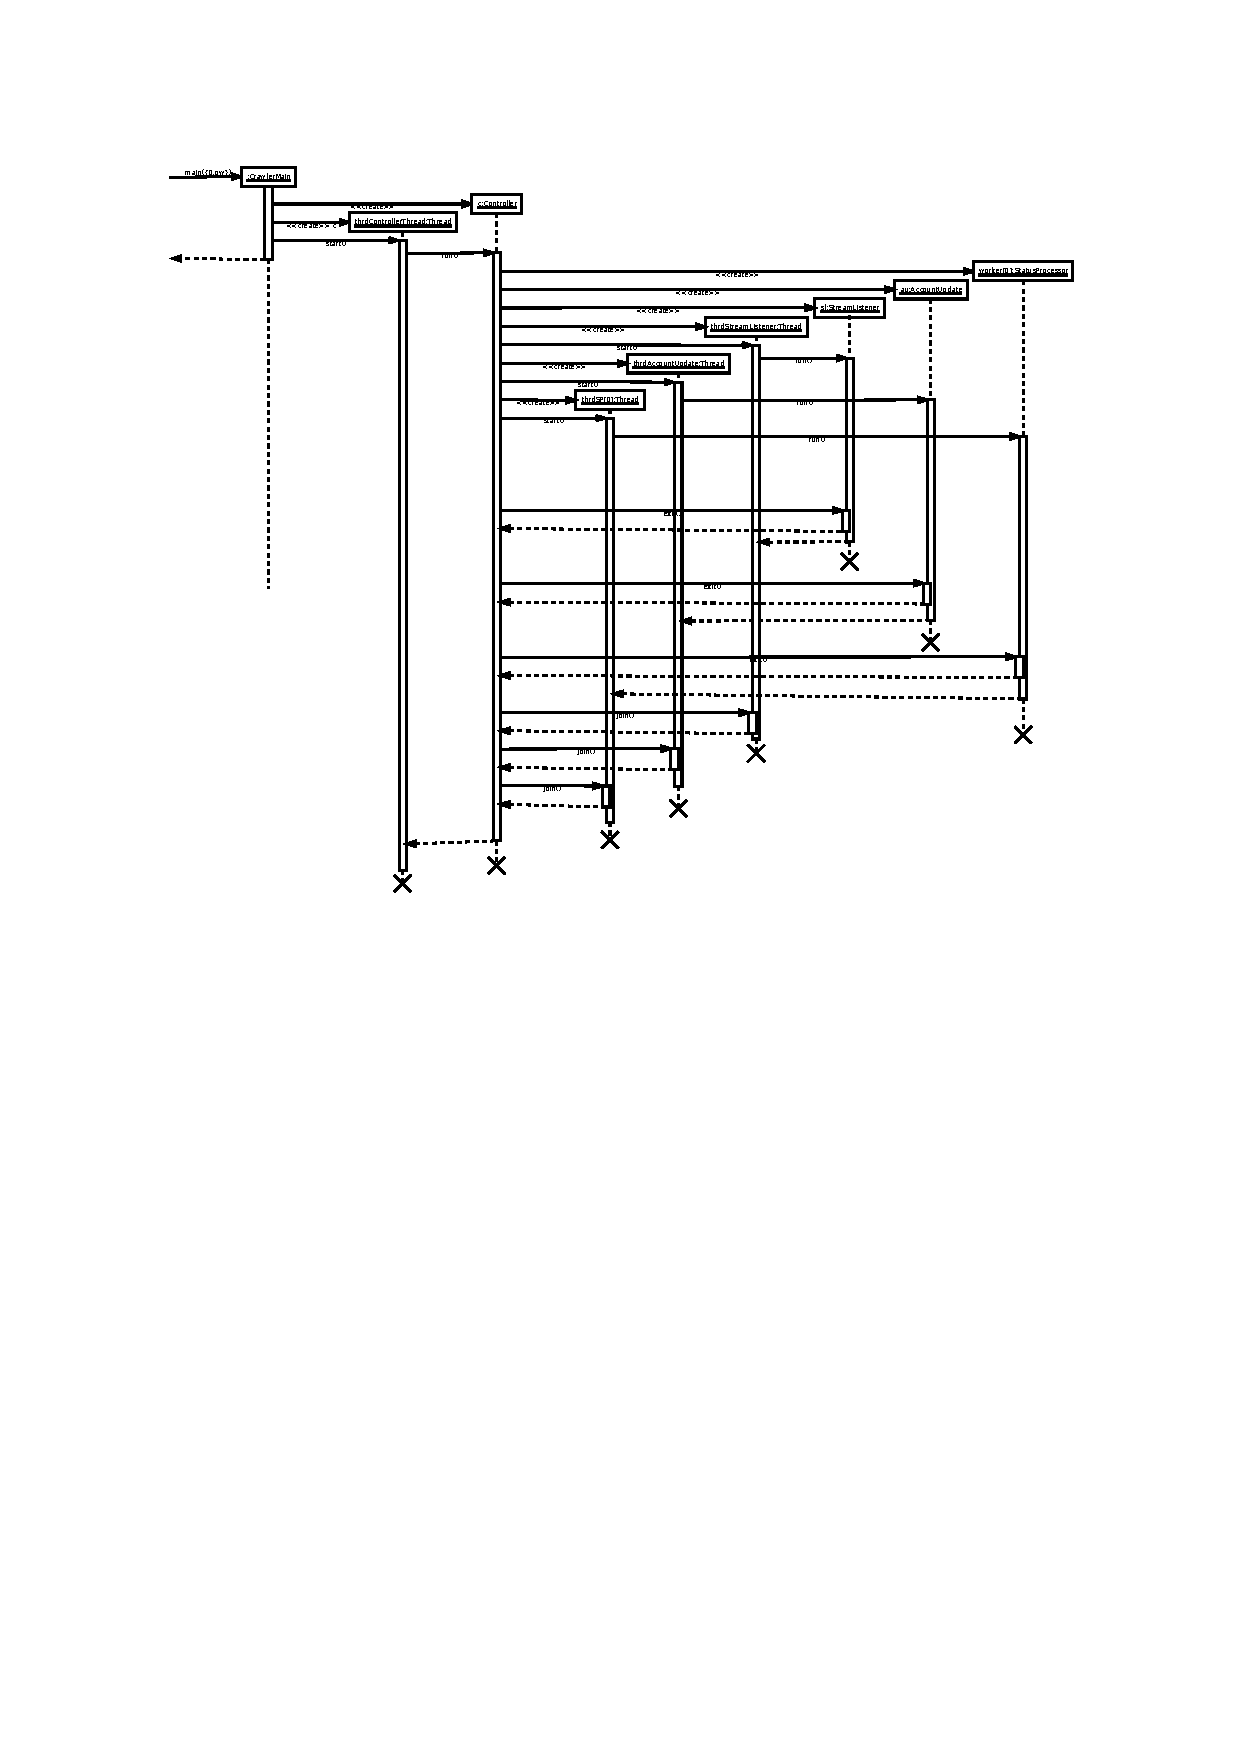
\includegraphics[width=\textheight,height=\textwidth,keepaspectratio=true,angle=-90]{dia/crawler_start_sequence}
	\caption{Sequenzdiagramm zum Start des Crawlers}
	\label{fig:crawler_start}
\end{figure}

Um den Crawler zu starten, werden ihm die Zugriffsdaten auf die Datenbank übergeben und die Anzahl der Threads die später Daten verarbeiten (Hardware abhängig).
Die main-Methode der Main-Klasse instantiiert daraufhin ein Controller Objekt, welches ab dann sämtliche Steuerung übernimmt. Diese Controller Objekt wird dann in einem Thread ausgeführt. Die Main-Klasse ist nun nur noch dafür zuständig Benutzereingaben entgegenzunehmen und diese weiter zu delegieren.
Sobald der Controller gestartet wurde instantiiert er die StatusProcessor Objekte, welche später sämtliche Daten verarbeiten müssen (deren Anzahl vom Benutzer festgelegt wird). Außerdem werden noch ein AccountUpdate- und ein StreamListener-Objekt instantiiert. Ersteres dient dazu eine Liste nicht verifizierter Accounts, die dennoch getracked werden sollen, aus der Datenbank aktuell zu halten. Zweiteres ist dafür zuständig eine Verbindung zur TwitterStream-API einzurichten. Alle diese Objekte werden dann vom Controller als eigenständige Threads ausgeführt.
Daraufhin beginnt der StreamListener eine Verbindung zur TwitterStreaming-API herzustellen (siehe \cref{fig:initialize_stream}).\\
Nun ist der Crawler im aktiven Zustand und empfängt Daten von Twitter, welche dann gefiltert, vervollständigt und in der Datenbank abgelegt werden.\\
Wird der Crawler vom Benutzer beendet, so sendet der Controller jedem Objekt, welches in einem Thread läuft ein exit-Signal. Daraufhin beenden die Objekte ihre Tätigkeit und der jeweilige Thread kehrt zum Controller zurück, sodass dieser dann das gesamte Programm beenden kann.
\\

\begin{figure}[h!]
	\centering
	\includegraphics[width=\textheight,height=\textwidth,keepaspectratio=true,angle=-90]{dia/crawler_initialize_stream}
	\caption{Sequenzdiagramm zur Initialisierung des TwitterStreams}
	\label{fig:initialize_stream}
\end{figure}

Um eine Verbindung zur Twitter-Streaming-API herzustellen, wird zuerst ein RateLimitStatusListener erstellt um auf Rate-Limits von Twitter zu reagieren. Danach wird noch ein Filter erstellt mit dem der Twitterstream durchsucht wird und ein MyStatusListener um über eingehende Daten benachrichtigt zu werden.
Anschließend wird ein TwitterStream-Objekt aus der twitter4j-Bibliothek geholt(ist Singleton). Auf diesem werden dann die Methoden zur Initialisierung aufgerufen und somit die Listener und der Filter gesetzt.\\
Zum Schließen des Streams wird auf dem TwitterStrem-Objekt die shutdown-Methode aufgerufen.

\section{Verarbeitung der Daten von Twitter}
Um zu verdeutlichen wie die Daten von Twitter innerhalb des Crawlers verarbeitet werden, ist in \cref{fig:crawler_process} der Datenfluss durch den Crawler exemplarisch dargestellt. Dabei werden die Daten von Twitter abgeholt, gepuffert, dann gefiltert und schlussendlich in die Datenbank geschrieben.

\begin{figure}[h!]
	\centering
	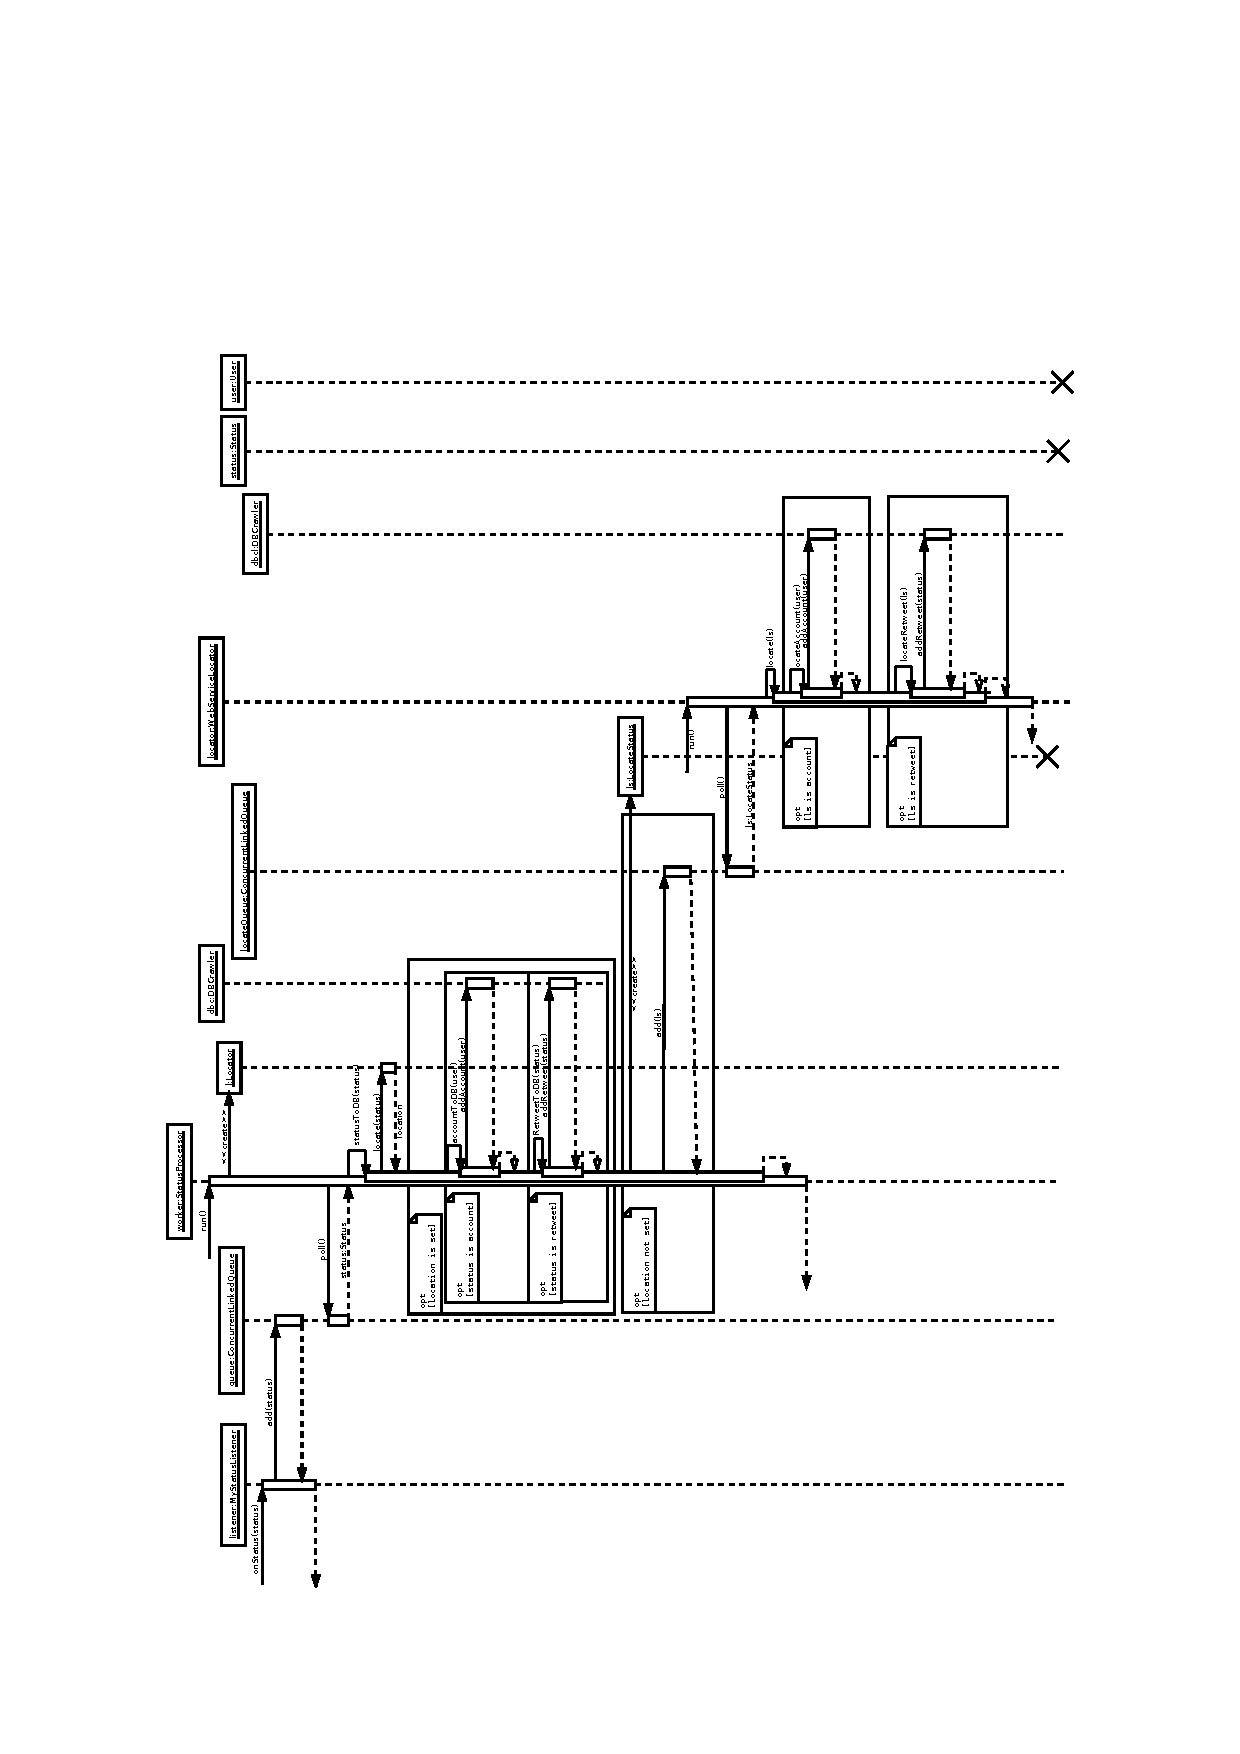
\includegraphics[width=\textheight,height=\textwidth,keepaspectratio=true,angle=-90]{dia/crawler_process_sequence}
	\caption{Sequenzdiagramm der Verarbeitung der Daten von Twitter}
	\label{fig:crawler_process}
\end{figure}

Im Folgenden soll der Weg der Daten von Twitter in unsere Datenbank mit \cref{fig:crawler_process} beschrieben werden.
Zuerst werden die Daten, welche im MyStatusListener auflaufen in eine (threadsichere) Warteschlange geschoben.
Hat dann ein StatusProcessor freie Kapazitäten so entnimmt er das erste Element der Warteschlange. Dieses Status-Objekt enthält alle relevanten Informationen um zu entscheiden ob das Objekt interessant ist oder nicht.
Interessante Status-Objekte enthalten verifizierte Twitter-Accounts oder Retweets auf Tweets von verifizierten Accounts. Ist ein verifizierter Account in einem Status-Objekt gefunden worden, so wird der Account (hier: user) dem Locator zur Lokalisierung übergeben. Dieser versucht dann anhand eines Orts-Strings den Account einem Land zuzuordnen. Ist dies geschehen so wird der Account in die Datenbank geschrieben. Genauso wird auch mit den Status-Objekten verfahren die einen Retweet enthalten.
Ist ein solches Status-Objekt verarbeitet, so beginnt der ganze Verarbeitungsprozess wieder von vorne.

	\chapter{Kategorisierer}
	\label{chap:kategorisierer}
		\section{Aufbau}
Der Kategorisierer wird in regelmäßigen Abständen vom Betriebssystem gestartet und verbindet sich mit der Datenbank. Über die Datenbankschnittstelle ließt er die bislang unkategorisierten Twitteraccounts aus der Accountstabelle aus und sucht in der DMOZ-Datenbank nach passenden Kategorien. Diese werden dann in die Kreuztabelle AccountCategory eingetragen.

Im Diagramm \ref{fig:categorizer} ist der grundlegende Aufbau des Kategorisierers dargestellt:
\begin{figure}[h!]
	\centering
	\includegraphics[width=\textwidth,height=\textheight, keepaspectratio=true]{dia/categorizer}
	\caption{Klassendiagramm des Kategorisierers}
	\label{fig:categorizer}
\end{figure}
\begin{description}
	\item[Account] siehe \cref{sec:datenbankzugriff}
	\item[Category] siehe \cref{sec:datenbankzugriff}
	\item[DBIcategorizer] Über dieses Interface kommuniziert der Kategorsierer mit der Datenbank. Es enthält Methoden zum Holen der unkategorisierten Accounts, zum Finden von Kategorien, zum Eintragen einer Kategorie und zum Auffinden aller Subkategorien einer Kategorie.
	\item[Categorizer] Dies ist die Haupt-Klasse des Kategorisierers. Sie nutzt die Methoden von \lstinline{DBIcategorizer}, um unkategorisierte Accounts zu suchen und gefundene Kategorien einzutragen.
\end{description}

\section{Start des Kategorisierers}
Der Kategorisierer soll in regelmäßigen Abständen vom Betriebssystem gestartet werden und daraufhin die neu gefundenen Accounts kategorisieren.

Der Ablauf des Kategorsierers ist im Sequenzdiagramm \ref{fig:categorizerSeq} zu sehen.
\begin{figure}[h!]
	\centering
	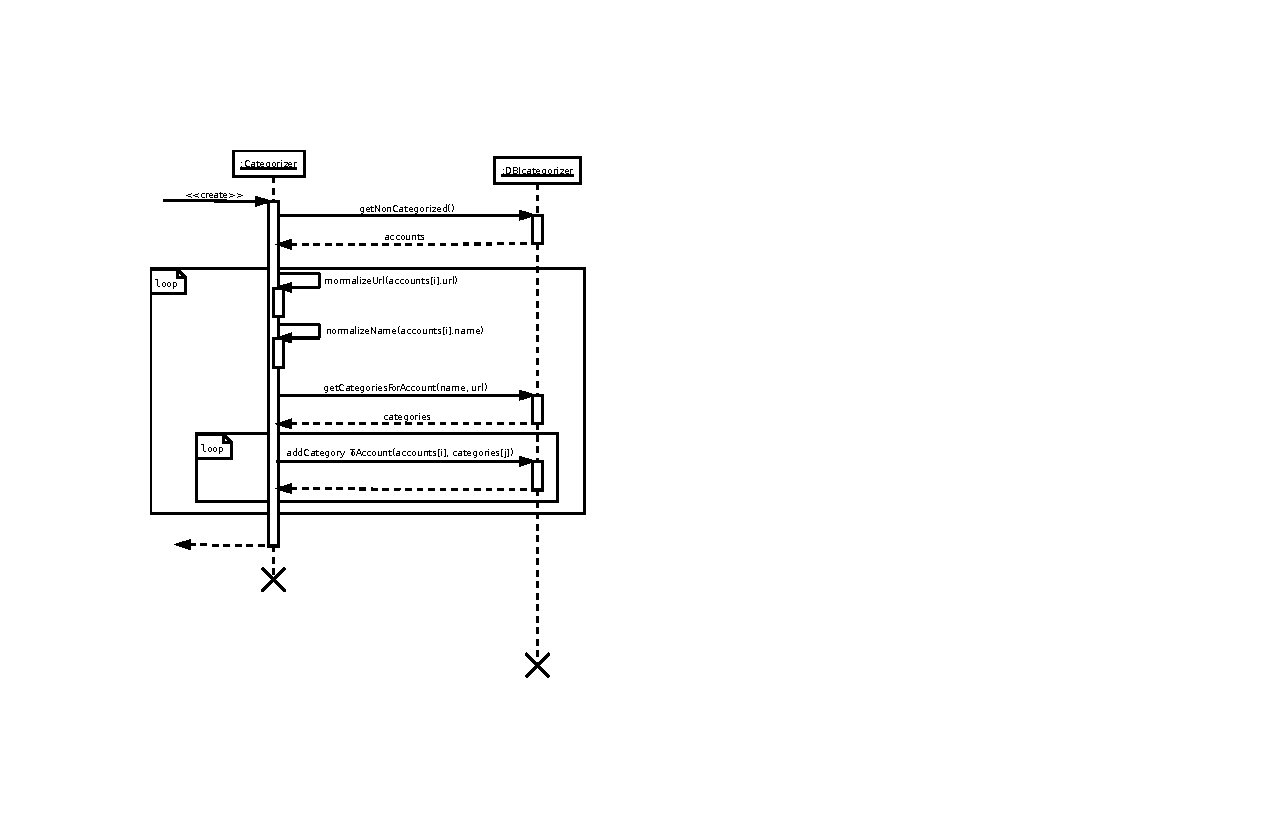
\includegraphics[width=\textwidth,height=\textheight,keepaspectratio=true]{dia/categorizerSequence}
	\caption{Sequenzdiagramm für einen Durchlauf des Kategorisierers. Dabei sind exemplarisch nur jeweils der erste unkategorisierte Account und die erste gefundene Kategorie aufgeführt.}
	\label{fig:categorizerSeq}
\end{figure}

Im ersten Schritt wird also eine Liste von unkategorisierten Accounts ausgelesen. Für jeden dieser Acounts wird eine Liste passender Kategorien ermittelt, die dann nach und nach in die Datenbank geschrieben werden.

	\chapter{GUI}
	\label{chap:gui}
		\section{Aufbau}
\subsection{Paketdiagramm}
\subsection{Klassendiagramm}
Die GUI ermöglicht die Interaktion des Benutzers mit der Anwendung und stellt die über den Crawler gesammelten Daten grafisch aufbereitet dar. 
\begin{figure}[h!]
	\centering
	\includegraphics[width=\textwidth,height=\textheight,keepaspectratio=true]{dia/TwitterGUI_Erweiterung}
	%\includegraphics[width=\textheight,height=\textwidth,keepaspectratio=true,angle=-90]{dia/TwitterGUI_Erweiterung}
	\caption{Klassendiagramm der GUI}
	\label{fig:GUI}
\end{figure}
\begin{description}
	\item[GuiController] Diese Klasse enthält alle GUI-Elemente. Damit kann über diese Klasse jedes einzelne Element angesprochen und damit gesteuert werden. Außerdem speichert sie die jeweils aktuellen Resultate der Datenbankabfragen zentral. Jede Erweiterung muss sich im GuiController als 'Observer' eintragen, um über Änderungen der Daten informiert zu werden. 
	\item[GuiElement] Interface, das jedes GUI-Element implementieren muss.
	\item [selectionOfQuery] Dieses Paket enthält Darstellung und Anwendungslogik für die Auswahl einer Suchanfrage (Auswahl von Kategorie, Land, usw.)
	\item[databaseOptions] Dieses Paket enthält die Darstellung und Anwendungslogik für Änderungen an der Datenbank, wie das Hinzufügen eines bisher nicht mitgetrackten Accounts.
	
	\item [standardMap] Das Paket enthält Anwendungslogik und Darstellung für die Standardkarte, welche die Länder nach dem jeweiligen Tweet-Retweet-Aufkommen einfärbt.
	\item [table] Paket, welches Anwendungslogik und Darstellung für die Erstellungen und Anzeige des Datenblattes zur aktuellen Anfrage enthält.
	\item [timeSliderMap] Paket, welches Anwendungslogik und Darstellung für Erstellung und Anzeige des Tweet-Retweet-Aufkommens in Abhängigkeit des gewählten Zeitraums anzeigt.
	\item [myUnfoldingMap] Diese Klasse kapselt die eigentliche Darstellung sämtlicher Kartenanzeigen. Sie ist die 'Schnittstelle' zur Unfolding-Library, welche für die Anzeige der Weltkarte verwendet wird.
\end{description}
\section{Sequenzdiagramme}
\subsection{GUI Initialisierung}
\begin{figure}[h!]
	\centering
	\includegraphics[width=\textwidth,height=0.5\textheight,keepaspectratio=true]{dia/GUISequenz_Start}
	\caption{Sequenzdiagramm der Initialisierung der GUI.}
	\label{fig:GUIStartSeq}
\end{figure}
\subsection{Kommunikation: GUI und Datenbank}
In \cref{fig:GUISeq} ist die Auswahl einer neuen Kategorie in einem Sequenzdiagramm dargestellt. Der Benutzer klickt auf eine Kategorie in der Liste, woraufhin \emph{handle(mouseEvent)} ausgelöst wird. Der \emph{SelectionOfQuerryController} gibt dieses Ereignis dem \emph{GuiController} weiter bzw. übergibt ihm eine Liste aller IDs ausgewählter Kategorien. Diese Klasse wiederum läd mittels \emph{getData} neue Daten zu den sich geänderten Kategorien. Die IDs ausgewählter Kategorien, Locations und Accounts (siehe Parameter der Operation \emph{getData}) sind dabei lokal in der Klasse \emph{GUIController} gespeichert.

Alle GUI-Elemente werden dann mittels \emph{update} über geänderte Daten informiert. Als Parameter wird ein Enum übergeben, der den Typ der Datenänderung angibt. Es gibt folgende Typen:
\begin{description}
	\item[TWEET] Die Information Anzahl Retweets pro Land und Tweet hat sich geändert. Hier ist bspw. eine Karte, die die Anzahl der Retweets pro Land graphisch darstellt, oder eine Tabelle mit vorher genannten Daten betroffen. 
	\item[CATEGORY] Eine lokale Liste der Kategorien wurde verändert. Die Liste, aus der der Benutzer Kategorien auswählt muss aktualisiert werden.
	\item[LOCATION] Länder bzw. Orte wurden aktualisiert. Auch hier ist z.B. die Liste im Filter, aus dem der Benutzer ein Land auswählt betroffen.
\end{description}
Bei Änderungen vom Typ \emph{TWEET} ist bspw. die \emph{StandardMapView} betroffen und fordert mittels \emph{getTweets()} die neue Informationen an und aktualisiert somit die aktuell angezeigte Karte. Einfachheitshalber wird hier nur die Aktualisierung eines GUI Elements visualisiert. Die Operation \emph{udpate} wird auf jedem GUI-Element, welches sich beim \emph{GUIController} mittels \emph{subscribe} angemeldet hat, aufgerufen.
\begin{figure}[h!]
	\centering
	\includegraphics[width=\textwidth,height=\textheight,keepaspectratio=true]{dia/TwitterGUI_Erweiterung_SequenzDiagramm}
	\caption{Sequenzdiagramm für Auswahl einer neuen Kategorie in der GUI.}
	\label{fig:GUISeq}
\end{figure}

	\chapter{Datenfluss}
	\label{chap:datenfluss}
		\section{Datenflussdiagramm}

Abschließend soll der Datenfluss innerhalb des Programms mithilfe von Abb. 6.1 genauer betrachtet werden.\\

\begin{figure}[h!]
	\centering
	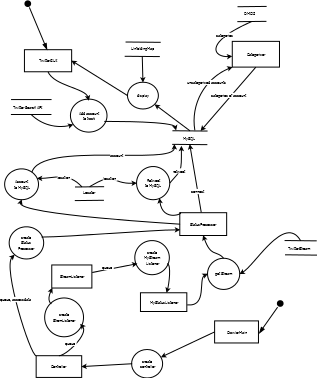
\includegraphics[width=\textwidth,height=0.8\textheight,keepaspectratio=true]{dia/datenflussdiagramm}
	\caption{Datenflussdiagramm des gesamten Systems}
	\label{fig:datenflussdiagramm}
\end{figure}

Der Datenfluss beginnt in der Klasse CrawlerMain, in der die main-Methode gestartet wird. Zuerst fließen dort Zugangsdaten der Datenbank an ein Controller Objekt, welche für seine Erzeugung notwendig sind. \\
Ist dies abgeschlossen werden mehrere StatusProssesor Objekte erzeugt denen jeweils die Queue, in der später die zu verarbeitenden Tweets enthalten sein werden, und Zugangsdaten für die Datenbank übergeben. Diese StatusProcessor Objekte verbinden sich anschließend mit Hilfe der zuvor erhaltenen Zugangsdaten mit der Datenbank. Zeitgleich wird ein StreamListener Objekt erzeugt dem wiederum die vorhin beschriebene Queue und ein Logger Objekt übergeben wird. Sobald diese Initialisierung abgeschlossen ist erzeugt das StreamListener-Objekt ein MyStreamListener, dem es wieder die Queue und einen Logger mitliefert. Sobald dies geschehen ist beginnt der MyStreamListener Daten aus dem TwitterStream auszulesen und sie in die Queue zu schreiben, die der StatusProcessor permanent bearbeitet. Solche Tweet-Objekte fließen also durch die Queue zu einer der StatusProcessor Instanzen. \\
Sobald ein StatusProcessor Objekt erkennt, dass der gerade in Bearbeitung befindlicheTweet von einem verifizierten Account kommt, wird der Account mit Hilfe der Daten, die der Kategorisierer liefert, (dieser benutzt dafür Daten aus der DMOZ-Datenbank) und der Daten, die der Lokalisierer liefert (dieser benutzt den Web-Lokalisierungsdienst), in die Datenbank geladen. Stellt der StatusProcessor fest, dass es ein Retweet war, wird er zusammen mit den Daten aus dem Lokalisierer in die Datenbank geladen.\\
Sind Daten in der Datenbank vorhanden können diese dann auf der TwitterGUI visualisiert werden. Dazu fließen die entsprechenden aufgearbeiteten Daten zusammen mit den notwendigen Daten die für die UnfoldingMap-Darstellung zur GUI. Werden nun in der GUI zusätzlilche Accounts zum Tracken angegeben, werden diese an die Datenbank gesendet und der Kreislauf wird geschlossen.\\
Die TwitterGUI ist somit ein zweiter Startpunkt für den Datenfluss.	
	%end{description}
	\chapter{Glossar}
		% Esentielle Begriffe.

\begin{description}

\end{description}

	\chapter{Größere UML Diagramme}
		% Detaillierte Beschreibung bestimmter für das Programm wichtige Abläufe anhand von Sequenzdiagrammen. Es sollten etwa 3-4 charakteristische und interessante Abläufe ausgewählt werden.

	\listoffigures
\end{document}

	\chapter{Softwarearchitektur}
		\input{include/architektur.tex}
	\chapter{Software}
		\input{include/software.tex}
\end{document}
